\documentclass[11pt]{standalone}

\usepackage{amssymb} 
\usepackage{amsmath} 

\usepackage[no-math]{fontspec}
\usepackage{unicode-math}
\setmainfont{TeX Gyre Heros}
\setmathfont{Stix Two Math}

\usepackage{xcolor}
\definecolor{darkblue}{HTML}{005A94}
\definecolor{lightblue}{HTML}{CCDEE9}
\definecolor{bgcolor}{HTML}{E5E7EB}

\usepackage{tikz}
\usetikzlibrary{arrows.meta, backgrounds}

\begin{document}
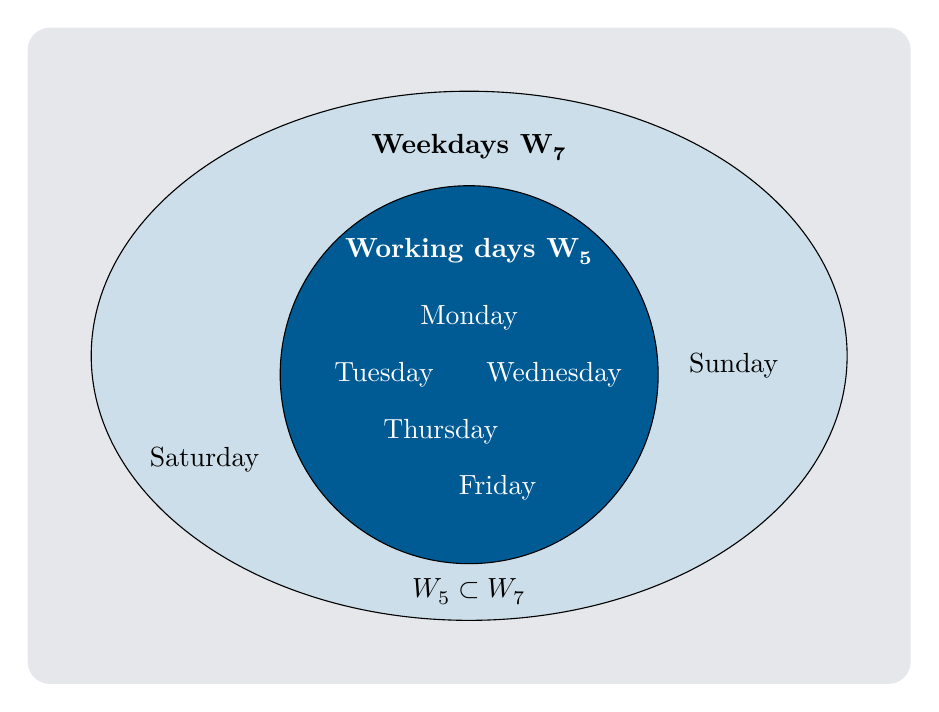
\begin{tikzpicture}[scale=1.2,
    show background rectangle,
    background rectangle/.style={fill=bgcolor, rounded corners=8pt},
    inner frame sep=0.8cm
]
  
  % Ellipse für Wochentage W_7
  \draw[fill=lightblue] (0,0) ellipse (4cm and 2.8cm);
  \node[font=\bfseries] at (0,2.2) {Weekdays $\mathbf{W_7}$};
  
  % Kreis für Werktage W_5 (innerhalb der Ellipse)
  \draw[fill=darkblue] (0,-0.2) circle (2cm);
  \node[font=\bfseries, white] at (0,1.1) {Working days $\mathbf{W_5}$};
  
  % Werktage innerhalb des Kreises
  \node[white] at (0,0.4) {Monday};
  \node[white] at (-0.9,-0.2) {Tuesday};
  \node[white] at (0.9,-0.2) {Wednesday};
  \node[white] at (-0.3,-0.8) {Thursday};
  \node[white] at (0.3,-1.4) {Friday};
  
  % Wochenende zwischen Ellipse und Kreis
  \node at (-2.8,-1.1) {Saturday};
  \node at (2.8,-0.1) {Sunday};
  
  % Teilmengensymbol
  \node at (0,-2.5) {$W_5 \subset W_7$};
  
\end{tikzpicture}
\end{document}